\documentclass[11pt]{article}
\usepackage[margin=1in]{geometry}
\usepackage{graphicx}
\usepackage{booktabs}
\usepackage{amsmath}
\usepackage{xcolor}
\usepackage{float}
\usepackage[hidelinks]{hyperref}
\usepackage{caption}
\captionsetup{font=small,labelfont=bf}
\usepackage{sectsty}
\definecolor{ohno}{HTML}{0072B2}
\definecolor{ssd}{HTML}{D55E00}
\sectionfont{\color{black!80}}
\newcommand{\ohno}{\textcolor{ohno}{\textbf{clustered cis-ohnolog}}}
\newcommand{\ssd}{\textcolor{ssd}{\textbf{clustered SSD-tandem}}}

\title{\textbf{CTCF binding architecture of clustered TF-paralog loci:\\
ohnolog vs.\ small-scale-duplication (tandem) clusters}}
\author{Iteration 19 --- Paralogous TF project\\\small ETS P01 genomics platform}
\date{2026-07-18}

\begin{document}
\maketitle

\begin{abstract}
\noindent We ask whether CTCF (insulator / TAD-boundary) binding differs between the two
\emph{clustered} classes of the iteration-16 four-group TF-duplication catalog:
\ohno{} loci (arising by whole-genome duplication) versus \ssd{} loci (tandem small-scale
duplications). Using a single ENCODE GM12878 CTCF ChIP-seq conservative-IDR peak set
(hg38), we profiled CTCF over each clustered locus extended by $\pm$100~kb. Both groups
are CTCF-enriched relative to the genome-wide expectation ($\sim$1.5--1.9$\times$ obs/exp),
and global CTCF density is statistically indistinguishable between them (Mann--Whitney~U,
all $p>0.7$). The one metric that separates the two groups is the \emph{number of CTCF peaks
lying between the two paralog members} (median 3 for ohnolog vs.\ 1 for SSD-tandem;
$p=0.0035$), but this difference is largely explained by the larger inter-member spacing of
ohnolog pairs: once normalized to inter-member distance, the per-kb CTCF density between
members is no longer significant ($p=0.27$). The interpretation is that ohnolog paralog
pairs are separated by \emph{more} insulator elements because they sit farther apart, not
because the intervening DNA is intrinsically denser in CTCF.
\end{abstract}

\section{Data and provenance}
\textbf{Duplication catalog (reused, not recomputed).} The four-group catalog was taken
verbatim from iteration~16 (\texttt{TF\_dup\_2x2\_classification.tsv}) together with the
clustered-locus coordinates (\texttt{clustered\_paralogs.noKRABHOX.tsv}); genome build
hg38 (GENCODE~v45 basic). Every cluster in the clustered file maps to a single, consistent
\texttt{dup\_class4} label (0 mixed clusters). This iteration analyses only the two
\emph{clustered} classes; dispersed classes are out of scope.

\textbf{CTCF peaks (one download).} ENCODE experiment \texttt{ENCSR000DZN}
(TF ChIP-seq, target CTCF, biosample GM12878, EBV-transformed B-lymphoblastoid),
file \texttt{ENCFF796WRU} --- \emph{conservative IDR-thresholded peaks}, \texttt{bed
narrowPeak}, assembly GRCh38, released. Downloaded 2026-07-18 from
\href{https://www.encodeproject.org}{encodeproject.org}. Sanity checks: 44{,}217 peaks;
chromosomes chr1--22 and chrX (no chrY, as expected for the female GM12878 line);
point-ish narrowPeak intervals. Accession and date are recorded in
\texttt{log/encode\_download.log} and in the script headers. GM12878 was chosen for its
lymphoid relevance to the project; the cell line is a CLI argument so a second line can be
swapped in later.

\section{Methods}
\textbf{Windows.} Each clustered locus was extended to
$[\texttt{cluster\_start}-100\,\text{kb},\ \texttt{cluster\_end}+100\,\text{kb}]$, clipped
to hg38 chromosome bounds (1 window shortened by clipping). One chrY locus (HSFY1/HSFY2,
SSD-tandem) was dropped because GM12878 carries no chrY signal and would contribute a
technical zero. Final set: \textbf{47} \ohno{} and \textbf{30} \ssd{} clusters (counts are
\emph{clusters}, not member TFs; caveat~ii).

\textbf{Binning.} Two representations were produced (caveat~iii). (A)~Fixed-width 5~kb bins
across the raw window (used only for the per-locus heatmap; bins do not align across loci of
different span). (B)~A length-normalized \emph{metagene}: the left 100~kb flank in 20
fixed-bp bins, the cluster body in 20 scaled bins, the right 100~kb flank in 20 fixed-bp
bins, on a relative-position axis $-1\!\to\!0$ (left flank), $0\!\to\!1$ (body),
$1\!\to\!2$ (right flank). The metagene is what is averaged and compared across loci.

\textbf{CTCF metrics.} Per bin: peak-summit count and bp-coverage fraction. Per locus:
CTCF peaks/kb over the window, body, and flanks; observed/expected ratio against the
genome-wide baseline ($44{,}217/3.03\,\text{Gb}=0.0146$ peaks/kb); distance of the nearest
CTCF peak to each member TSS; and the count of CTCF peaks between the outermost member TSSs
(both raw and normalized per kb of inter-member distance).

\textbf{Statistics (reproducibility rule).} Two-sided \textbf{Mann--Whitney~U},
\ohno{} vs.\ \ssd{}, on each per-locus continuous metric (report $U$, $p$, per-group $n$ and
medians, rank-biserial effect size $r_{rb}$). Metagene profiles carry bootstrap 95\% CI
bands (2000 resamples). A per-bin Mann--Whitney~U across the 60 metagene bins was run with
Benjamini--Hochberg FDR to localize any positional difference.

\section{Results}

\subsection*{Both clustered classes are CTCF-enriched, and globally indistinguishable}
Over the $\pm$100~kb window both groups carry CTCF well above the genome-wide expectation
(median obs/exp $1.70$ ohnolog, $1.52$ SSD-tandem). None of the global density metrics
separate the groups (Table~\ref{tab:mwu}; all $p>0.70$), and the metagene profiles overlap
within their bootstrap CI bands across the whole window (Fig.~\ref{fig:metagene}); \textbf{0
of 60} metagene bins reach BH-FDR $<0.05$. In short, at the level of overall insulator
density the two kinds of clustered loci occupy statistically similar CTCF environments.

\begin{table}[H]
\centering
\small
\caption{Per-locus CTCF metrics, \ohno{} ($n=47$) vs.\ \ssd{} ($n=30$).
Two-sided Mann--Whitney~U. $r_{rb}$ = rank-biserial effect size
(negative $\Rightarrow$ ohnolog $>$ SSD-tandem).}
\label{tab:mwu}
\begin{tabular}{lrrrrr}
\toprule
Metric & median (ohnolog) & median (SSD) & $U$ & $p$ & $r_{rb}$ \\
\midrule
CTCF peaks/kb, window        & 0.0248 & 0.0222 & 695.0 & 0.921 & $+0.014$ \\
CTCF peaks/kb, locus body    & 0.0238 & 0.0332 & 668.0 & 0.703 & $+0.053$ \\
CTCF peaks/kb, flanks        & 0.0250 & 0.0225 & 695.0 & 0.921 & $+0.014$ \\
Observed/expected, window    & 1.702  & 1.521  & 695.0 & 0.921 & $+0.014$ \\
Nearest CTCF to a TSS (bp, min)  & 4241 & 1885 & 769.5 & 0.504 & $-0.092$ \\
Nearest CTCF to TSS (bp, mean)   & 11909 & 13727 & 687.0 & 0.855 & $+0.026$ \\
\textbf{CTCF peaks between members} & \textbf{3.0} & \textbf{1.0} & \textbf{981.5} & \textbf{0.0035} & $\mathbf{-0.392}$ \\
Inter-member TSS distance (bp)   & 74355 & 49409 & 866.0 & 0.094 & $-0.228$ \\
CTCF peaks/kb between members (norm.) & 0.0232 & 0.0178 & 809.5 & 0.274 & $-0.148$ \\
\bottomrule
\end{tabular}
\end{table}

\subsection*{Ohnolog members are separated by more CTCF peaks --- a spacing effect}
The single metric that distinguishes the groups is the number of CTCF peaks \emph{between}
the two paralog members: ohnolog pairs have a median of 3 intervening CTCF peaks versus 1 for
SSD-tandem pairs (Mann--Whitney~U, $p=0.0035$, $r_{rb}=-0.39$; Fig.~\ref{fig:between}, left).
However, ohnolog members also sit farther apart (median inter-member TSS distance 74~kb vs.\
49~kb, $p=0.09$). When the between-member CTCF count is normalized to inter-member distance,
the difference is no longer significant (0.023 vs.\ 0.018 peaks/kb, $p=0.27$;
Fig.~\ref{fig:between}, right). The extra insulator load between ohnolog paralogs is
therefore best read as a consequence of their wider genomic separation rather than an
intrinsically CTCF-denser intervening region --- consistent with ohnolog pairs, retained from
whole-genome duplication, having drifted farther apart than recent tandem duplicates while
remaining within the same broadly insulated neighbourhood.

\begin{figure}[H]
\centering
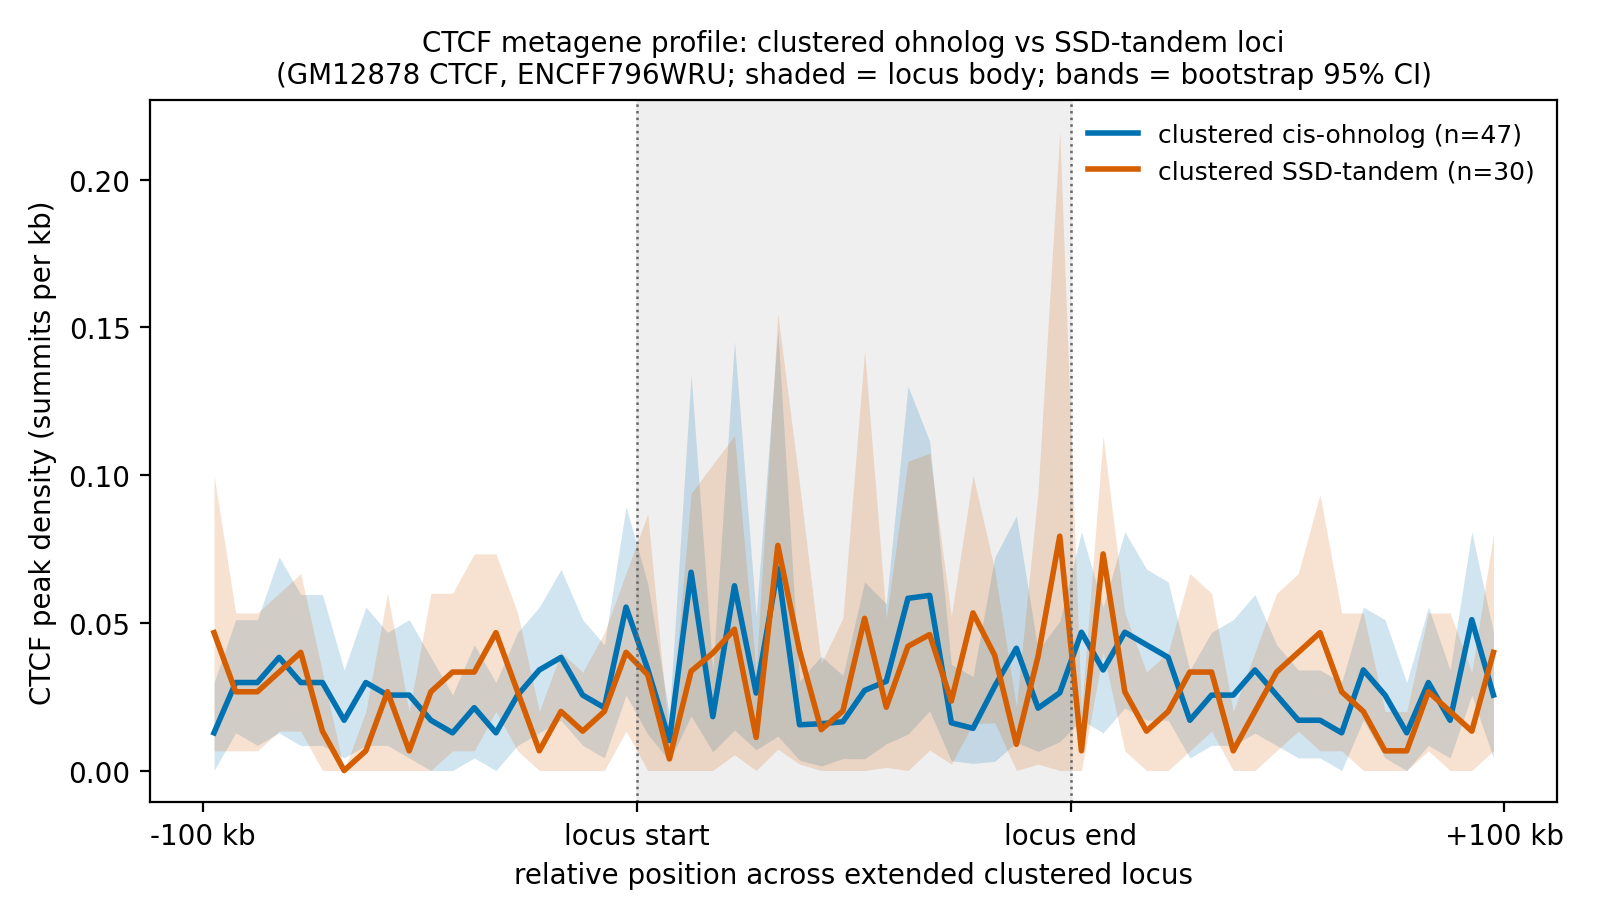
\includegraphics[width=0.92\textwidth]{../results/figures/ctcf_metagene_clustered_groups.png}
\caption{Length-normalized CTCF metagene profile. Lines = mean CTCF summit density per kb;
shaded bands = bootstrap 95\% CI; grey = locus body. The two clustered classes overlap
throughout; no metagene bin survives BH-FDR $<0.05$.}
\label{fig:metagene}
\end{figure}

\begin{figure}[H]
\centering
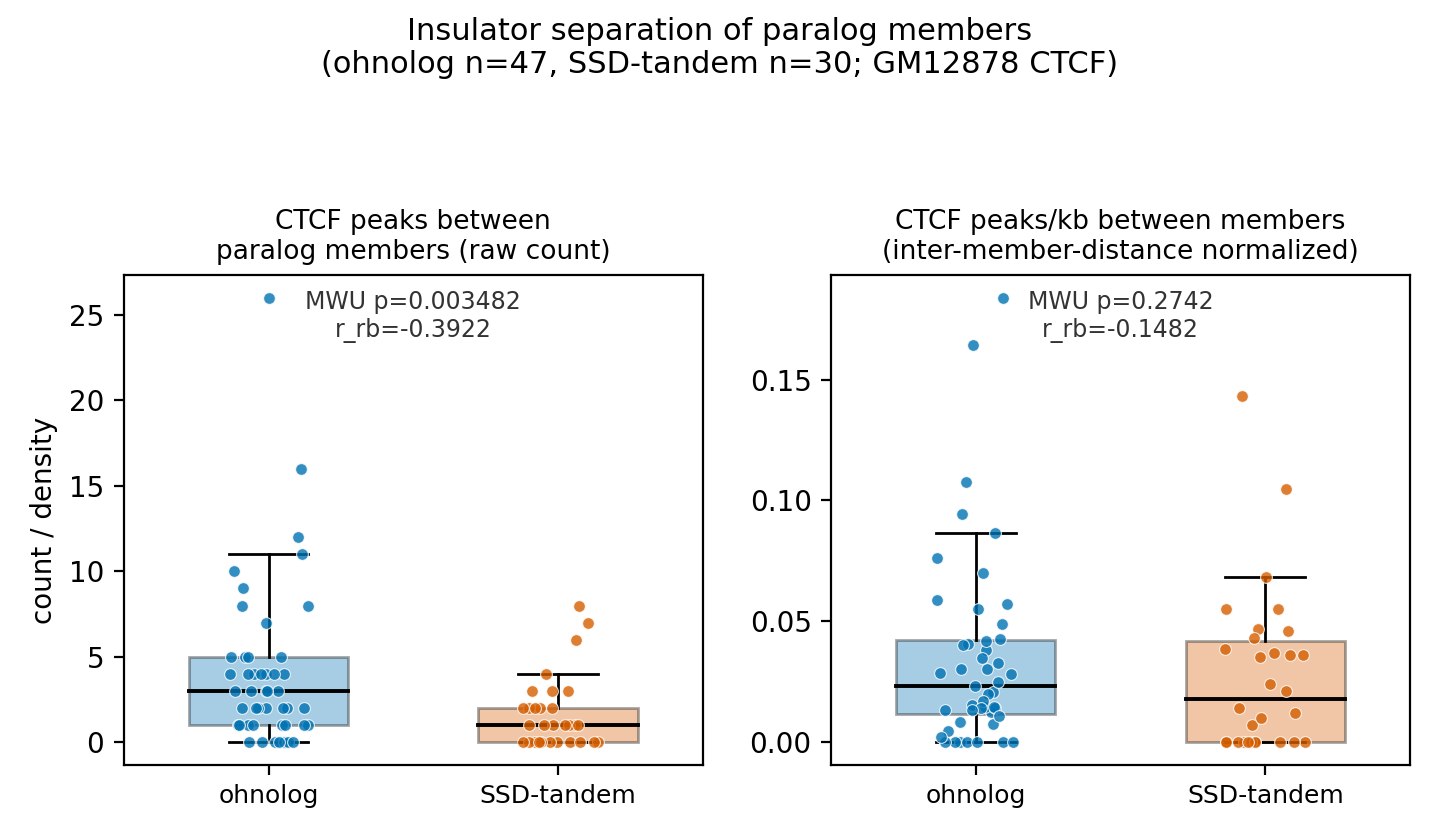
\includegraphics[width=0.75\textwidth]{../results/figures/ctcf_between_members.png}
\caption{CTCF insulator separation of paralog members. Left: raw count of CTCF peaks between
the two members differs (MWU $p=0.0035$). Right: after normalizing to inter-member distance
the per-kb difference is not significant ($p=0.27$), indicating the raw effect is driven by
the wider spacing of ohnolog pairs.}
\label{fig:between}
\end{figure}

\begin{figure}[H]
\centering
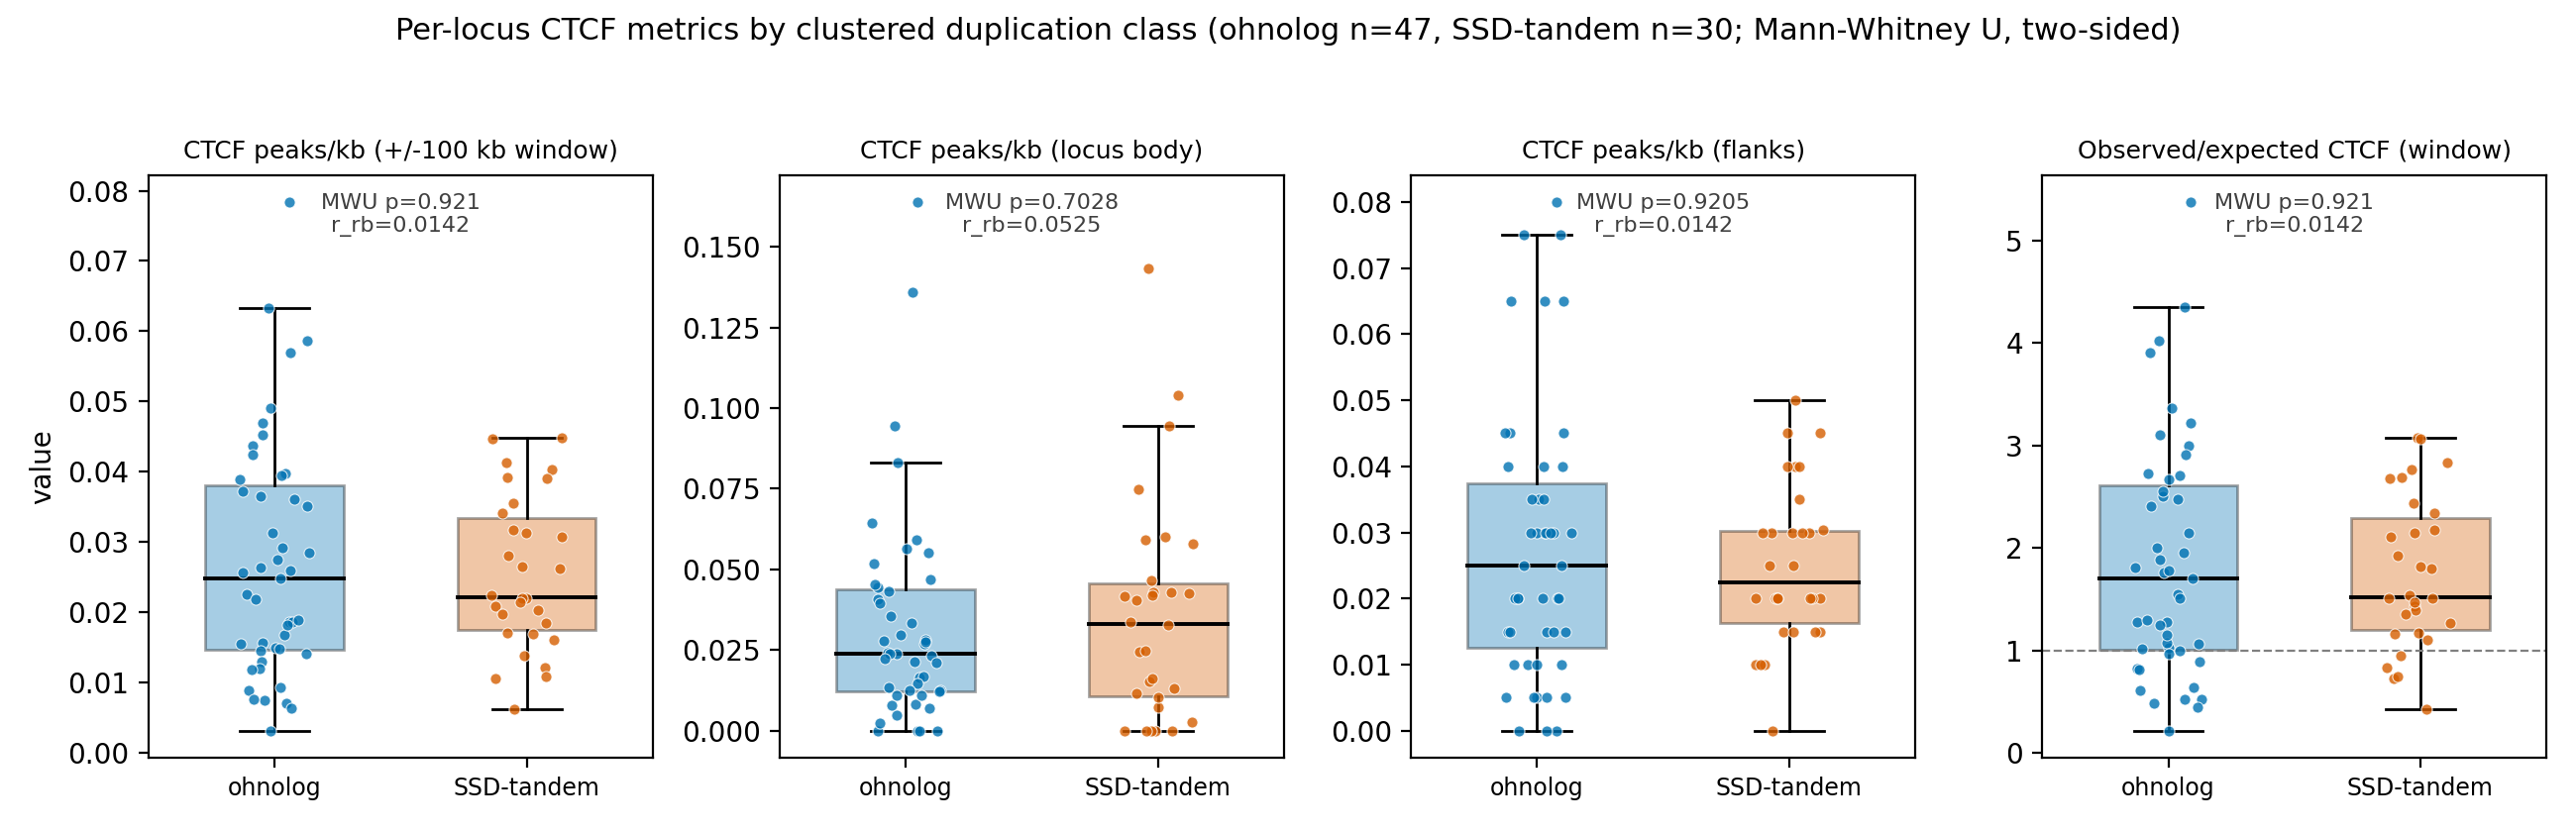
\includegraphics[width=0.98\textwidth]{../results/figures/ctcf_peaks_per_kb_by_group.png}
\caption{Per-locus CTCF density metrics by class (box + jittered points). All four global
metrics are indistinguishable between ohnolog and SSD-tandem loci; both groups exceed the
genome-wide expectation (dashed line = obs/exp $=1$).}
\label{fig:box}
\end{figure}

\begin{figure}[H]
\centering
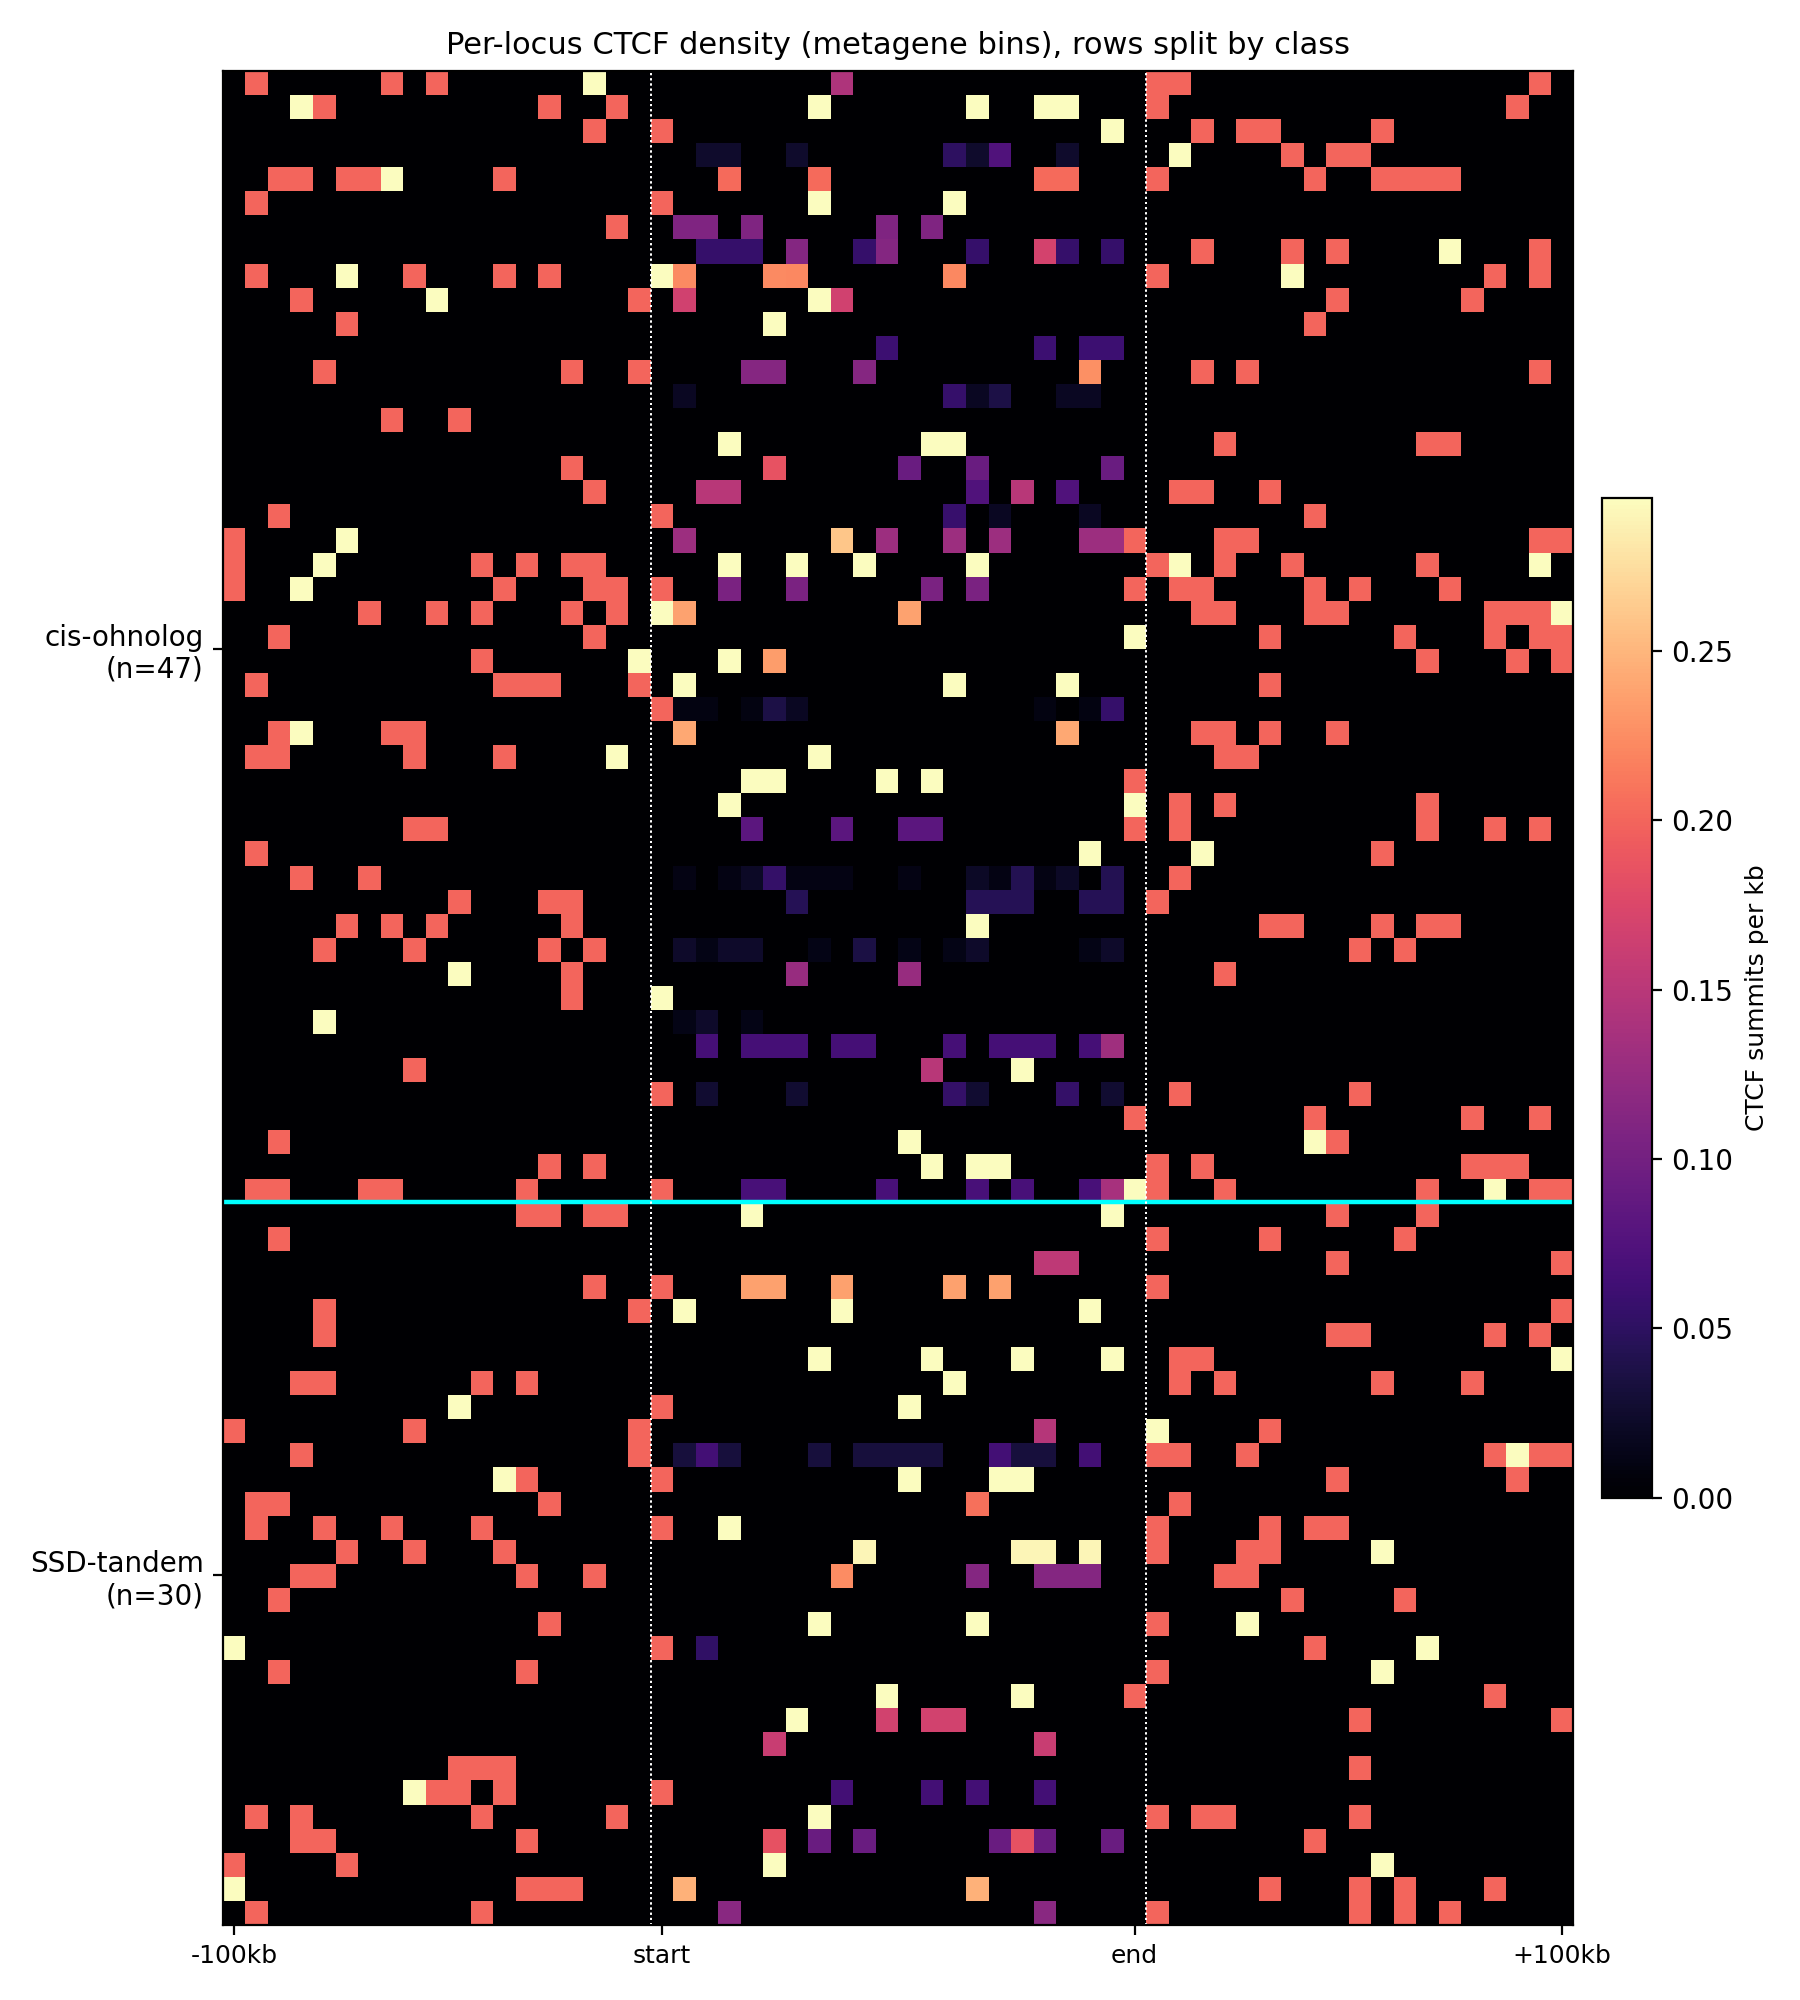
\includegraphics[width=0.62\textwidth]{../results/figures/ctcf_perlocus_heatmap.png}
\caption{Per-locus CTCF density across metagene bins, rows split by class (cyan line). CTCF
signal concentrates in and around the locus body in both groups without an obvious
class-specific pattern.}
\label{fig:heat}
\end{figure}

\section{Conclusion}
In GM12878, clustered ohnolog and clustered SSD-tandem TF-paralog loci occupy
\emph{statistically similar} CTCF insulator environments: both are CTCF-enriched over the
genome-wide background and their overall peak densities, flank/body distributions, and
TSS-proximal CTCF are indistinguishable. The only separating signal --- more CTCF peaks
between ohnolog members --- is accounted for by the greater physical distance between ohnolog
paralogs and does not survive distance normalization. Within the power available (47 vs.\ 30
clusters) we find no evidence that the two clustered duplication mechanisms sit in distinct
CTCF/insulator architectural niches.

\paragraph{Caveats.} (i)~A single cell type (GM12878); CTCF is largely constitutive but not
identical across lineages --- results are conditioned on this line. (ii)~Small groups
(47 vs.\ 30 clusters after collapsing members to \texttt{cluster\_id}); per-locus tests are
underpowered, and the borderline inter-member-distance trend ($p=0.09$) may reflect this.
(iii)~Fixed-bp binning and length-normalized metagene binning are reported separately, as
they are not comparable across loci of different span. (iv)~Extended windows can overlap for
nearby clusters and can run off chromosome ends; one window was clipped, and the single chrY
locus was excluded (no chrY signal in the female GM12878 line).

\end{document}
